%----------------------------------------------------------------------------
\chapter{Irodalomkutatás}\label{sect:Literature}
%----------------------------------------------------------------------------
\section{Mi is a Gantt diagramm?}

\hspace{2mm} Az amerikai származású gépész mérnök Henry Gantt-tól származik a nevét is örző Gannt diagramm forma. Ma már a projektmenedzsment mindennapjait kiséri végig ez a feladatok ütemezését vizuálisan megragadó eszköz. Maga a diagram egy elfektetett oszlopdiagramhoz hasonlít, amelyen követhetjük a projekthez tartozó egyes feladatok elvégzésének egy ütemezését. \listref{GanttChart} Két nagyobb megjelenítendő részből áll, egy a feladatokat listázza, egy pedig a naptárszerű rész mely az elvégzési ütemtervet mutatja. 

\begin{figure}[!ht]
\centering
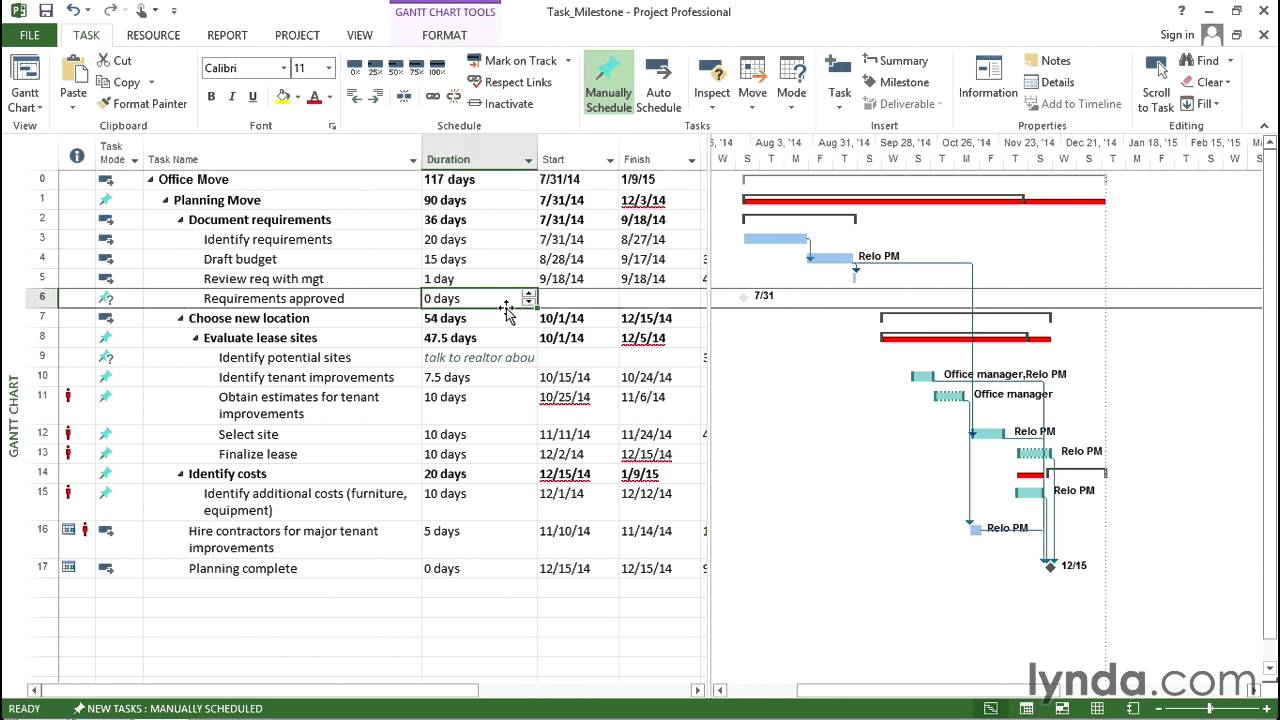
\includegraphics[width=\textwidth, keepaspectratio]{figures/msproject.jpg}
\caption{Microsoft Project 2016 Gantt program kinézete} 
\label{fig:MSProject}
\end{figure} 

A Microsoft Project által megvalósított Gantt vastag kliens alkalmazásra mutat példát a \figref{MSProject}-es ábra. Az ábrán megfigyelhetők a taskok legfontosabb tulajdonságai. Minden tasknál beállíthatjuk, hogy mennyi ideig fog tartani és, hogy milyen függöségei vannak, ezután a task kezdési és végzési idejét az alkalmazás az ütemezés függvényében állítja majd be. Láthatjuk, hogy nem csak feladatok vannak, hanem azoknak egy öszefoglalója, summaryje is melyek alá több feladat tartozhat. Fontos, hogy ez a summary nem egy külön task, hanem azoknak egy gyűjtője, az elvégzési időtartama is az alatta lévő taskok összege. Még érdemes azt is megemlíteni, hogy a program a taskok egymásutániságát nyílakkal is szemlélteti a jobb érthetőség és vizualizáció érdekében. \listref{MsProject}

A Microsoft Project ellenpontjaként több projekt próbálta vékonykliensen is megvalósítani az alkalmazást egy webes applikáció keretében, ilyen például a GanttPro, melyben a Microsoft Project legtöbb funkciója implementálásra került. A programba a \figref{GanttPro} ábra nyújt betekintést, feladatom a félév során egy ehhez hasonló alkalmazás alapjainak lefektetése volt.\listref{GanttPro}

\begin{figure}[!ht]
\centering
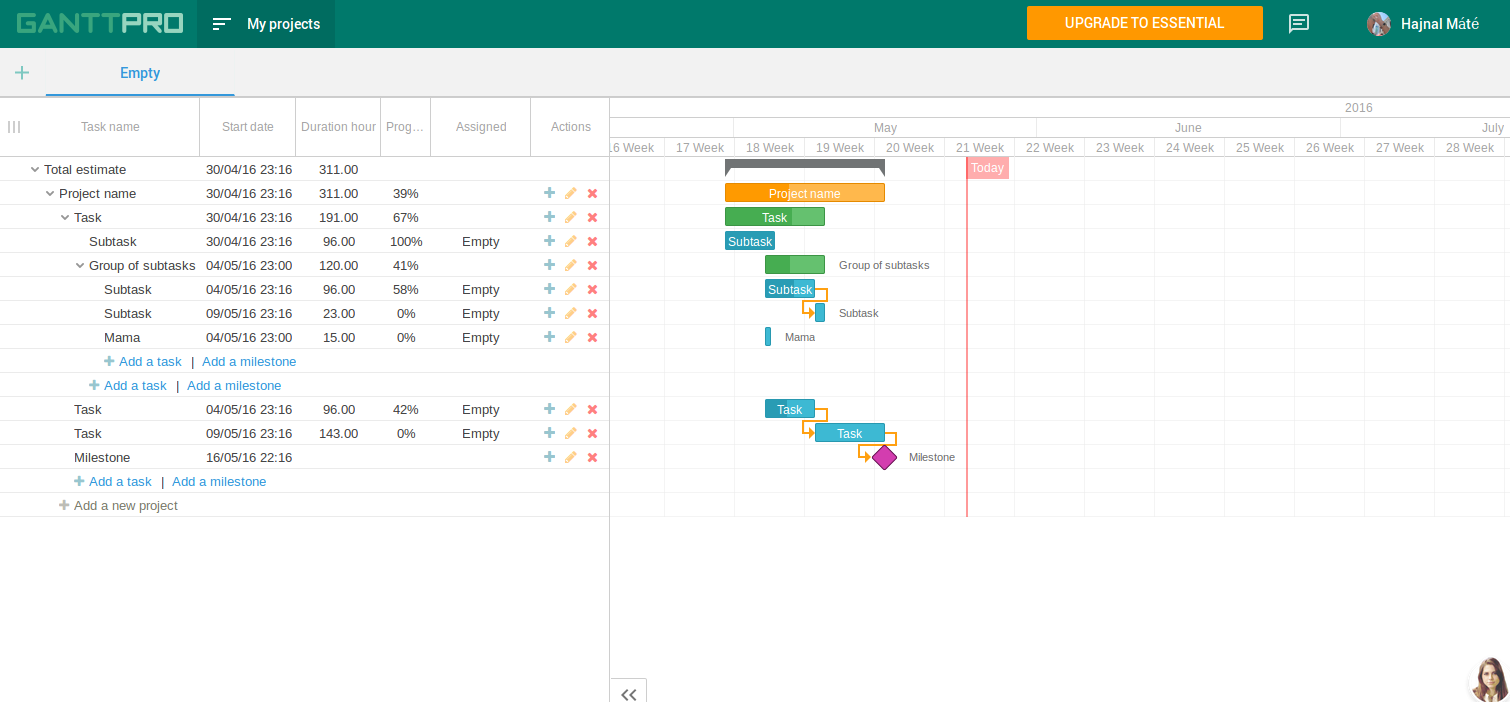
\includegraphics[width=\textwidth, keepaspectratio]{figures/ganntpro.png}
\caption{A GanttPro webes alkalmazás} 
\label{fig:GanttPro}
\end{figure} 

%----------------------------------------------------------------------------
\section{Critical Path Method}


%----------------------------------------------------------------------------
\section{Least Slack Time scheduling}
